\subsection{Orden del repositorio}
El repositorio se encuentra en \href{https://github.com/0-0REL/Dron}{GitHub} y se divide en tres ramas
\dirtree{%
.1 Dron.
.2 main\DTcomment{\#Rama principal}.
.3 ArduPilot/\DTcomment{Desarrollo con el AMP2.6}.
.4 bash scripts/\DTcomment{Scripts para iniciar GCS o simulación}.
.4 Dron/\DTcomment{Logs de pruebas de vuelo}.
.4 MAVLink/\DTcomment{Pruebas con MAVLink}.
.4 MP Python scripts/\DTcomment{Pruebas con scripts de Mission Planner}.
.4 sik-radio-config/\DTcomment{Reconfiguración de radios}.
.4 simulaciones/\DTcomment{Resultados de simulaciones del articulo}.
.3 Complementos/\DTcomment{Software auxiliar}.
.4 CAD\DTcomment{Modelos 3D en Inventor}.
.4 Modelos/\DTcomment{Modelos para Detección}.
.3 doc/\DTcomment{Este archivo}.
.3 MATLAB/\DTcomment{Simulacion en simulink y desarrollo de controladores}.
.4 control\_pid/.
.4 simmat/.
.4 simulink/.
.3 Navio2/\DTcomment{Logs de dron con Navio2}.
.4 magnetometro/\DTcomment{Calibración de magnetómetro}.
.4 ROS/.
.4 visualizacion/\DTcomment{Visualizar orientación}.
.3 OpenCV/.
.4 prototipo/\DTcomment{Versión funcional}.
.4 pruebas/.
.3 TensorFlow/\DTcomment{Entrenamiento de modelo de reconocimiento}.
.4 dataset/.
.2 apm-ros-jazzy\DTcomment{\#Rama con paquetes ROS-Jazzy para simulación}.
.3 mav\_ctrl/.
.3 vision/.
.2 ros-pkg-navio\DTcomment{\#Rama con paquetes ROS-Noetic para navio2}.
.3 navio2/\DTcomment{Procesamiento de sensores}.
.3 sys\_ctrl/\DTcomment{Controlador de vuelo}.
.3 vision/\DTcomment{Detección de rostros}.
}

El HAT Navio2 es compatible con las Raspberry Pi 2, 3 y 4. La imagen del sistema necesaria se encuentra \href{https://docs.emlid.com/navio2/configuring-raspberry-pi/}{aquí}. El sistema no tiene interfaz gráfica y funciona en arquitectura armv7l.

Para poder establecer un acceso remoto al Raspberry del dron incluso fuera de red local, se puede usar el servicio VPN de \href{https://tailscale.com/kb/1017/install}{Tailscale.}
\subsection{Componentes del cuadricóptero}
El dron cuenta con los siguientes componentes:
\begin{itemize}
	\item 4 Motores sin escobillas (BLDC)
	\item 4 Control de velocidad electrónico (ESC)
	\item 1 Batería LiPo 11.1 V
	\item 1 Computadora de vuelo, cuenta con:
	\begin{itemize}
		\item IMU (acelerómetro, giroscopio y magnetómetro)
		\item Barómetro
	\end{itemize}
	\item 1 Chasis
	\item 2 Helices CW
	\item 2 Helices CCW
\end{itemize}
\subsection{Control del cuadricóptero}
El dron utiliza un marco X y el orden de los motores asi como su dirección de giro se puede ver en la figura \ref{fig:marco}. 
\begin{figure}[H]
	\centering
	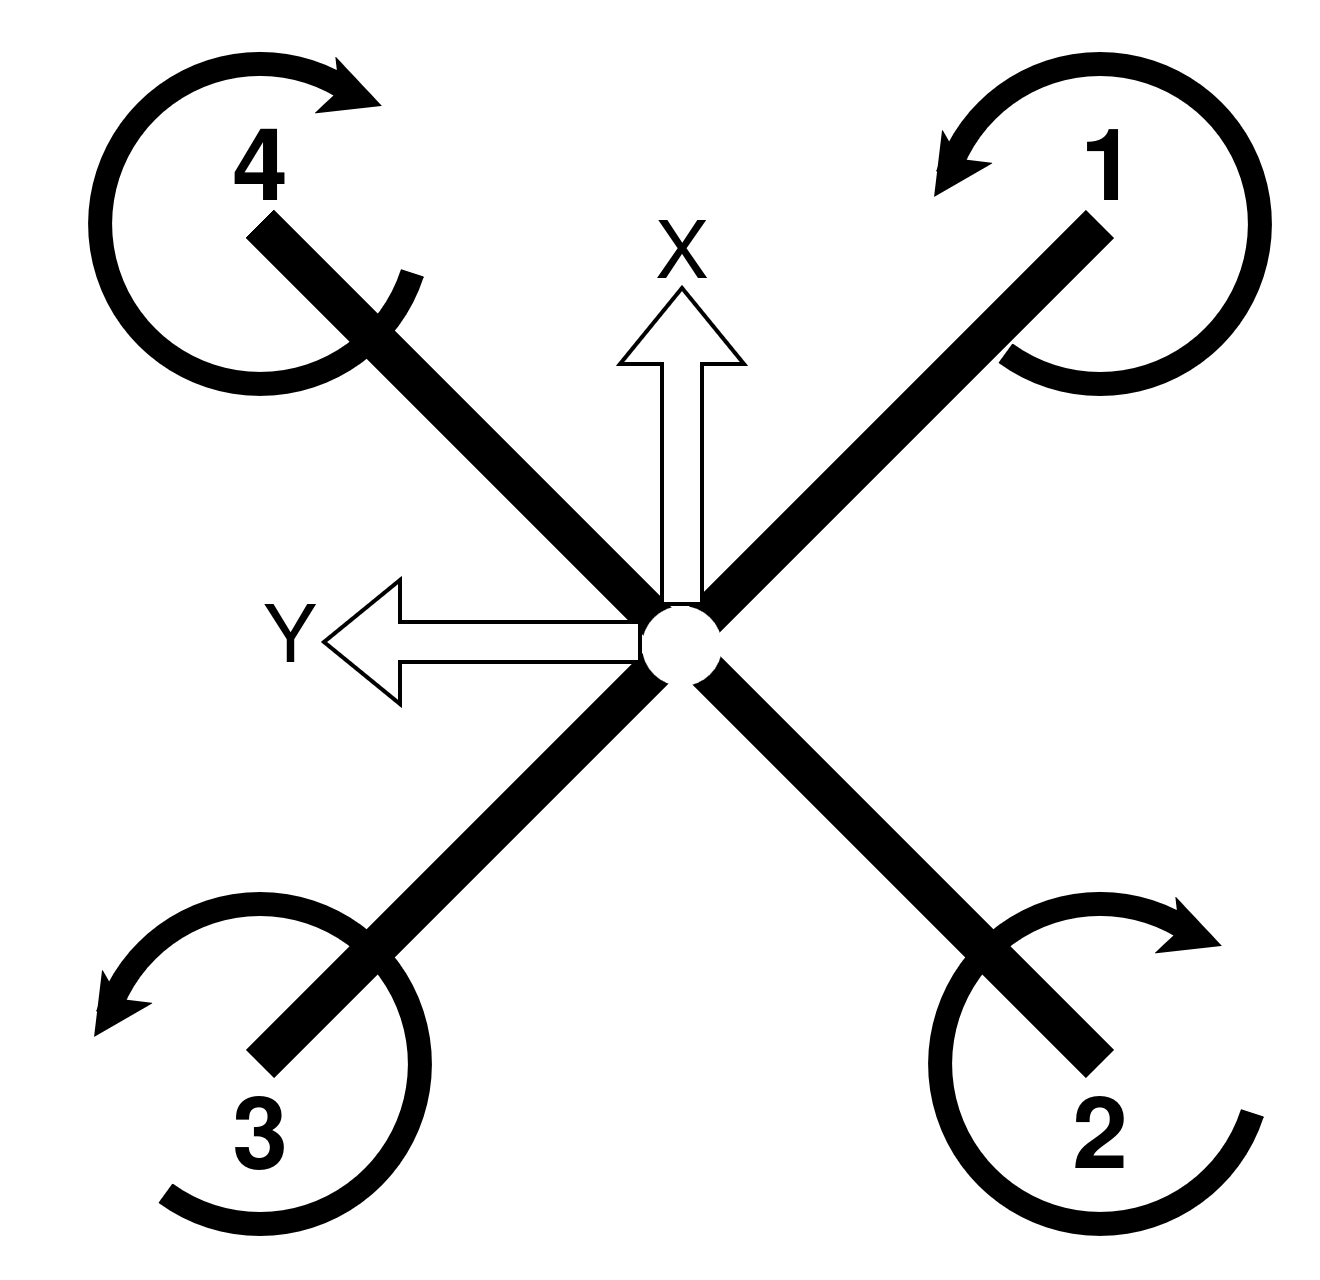
\includegraphics[width=4cm]{Imagenes/marco.png}
	\caption{Marco}
	\label{fig:marco}
\end{figure}
El par y empuje generados por cada motor están dados por:
\begin{gather}
	F_i = K_F \omega_i^2 \label{eq:kfomega}\\
	\tau_i = K_M \omega_i^2 \label{eq:kmomega}
\end{gather}
De modo que la relación entre la acción de cada motor y las entradas de control se relacionan de la siguiente forma
\begin{equation}
	\label{eq:mot2u}
	\begin{bmatrix}
		F\\
		\tau_x\\
		\tau_y\\
		\tau_z
	\end{bmatrix}
	=
	\left[\begin{array}{cccc}
	K_F  & K_F  & K_F  & K_F \\
	-K_F \,L & -K_F \,L & K_F \,L & K_F \,L\\
	-K_F \,L & K_F \,L & K_F \,L & -K_F \,L\\
	-K_M  & K_M  & -K_M  & K_M 
	\end{array}\right]
	\begin{bmatrix}
		\omega_1^2\\
		\omega_2^2\\
		\omega_3^3\\
		\omega_4^2
	\end{bmatrix}
\end{equation}

El modelo dinámico del dron se puede linealizar el modelo del dron mediante la serie de Taylor \cite{powersQuadrotorKinematicsDynamics2015}
\begin{equation}
	\label{eq:taylor}
	\dot{\mathbf{x}} = f(\mathbf{x,u})_{\mathbf{x0,u0}}+\left.\frac{\partial}{\partial \mathbf{x}} f(\mathbf{x}, \mathbf{u})\right|_{(\mathbf{x}_0, \mathbf{u}_0)} (\mathbf{x} - \mathbf{x_0})
	+
	\left.\frac{\partial}{\partial \mathbf{u}} f(\mathbf{x}, \mathbf{u})\right|_{(\mathbf{x}_0, \mathbf{u}_0)} (\mathbf{u} - \mathbf{u_0})
	=\mathbf{Ax + Bu} 
\end{equation}
\[\mathbf{x_0} = \mathbf{0}_{12\times1}\]
\[\mathbf{u_0} = \begin{bmatrix} mg & 0 & 0 & 0 \end{bmatrix}^T\]

El modelo en espacio de estados se puede convertir a funciones de trasferencia mediante
\begin{equation}
	\label{eq:ss2tf}
	\mathbf{G(s)} = \mathbf{C} \left[s\mathbf{I - A}\right]^{-1} \mathbf{B + D}
\end{equation}

El controlador PD tiene la siguiente estructura
\begin{equation}
	\label{eq:c_pd}
    PD(s) = K_P + K_D s = K_D(s+a)
\end{equation}
\[K_P = a K_D\]

El controlador PID tine la siguiente estructura
\begin{equation}
	\label{eq:c_pid}
    PID(s) = K_P + \frac{K_I}{s}+ K_D s = K_D\frac{(s+a)(s+b)}{s}
\end{equation}
\[K_I = abK_D\]
\[K_P= (a+b)K_D\]

Modelo Interno para entrada escalón \cite{dorfInternal2022}
\begin{equation}
	\label{eq:c_mi}
	\begin{bmatrix}
		\dot{\mathbf{e}}(t) \\
		\dot{\mathbf{z}}(t)
	\end{bmatrix}
	=
	\begin{bmatrix}
		0 & \mathbf{C} \\
		0 & \mathbf{A}
	\end{bmatrix}
	\begin{bmatrix}
		\mathbf{e}(t) \\
		\mathbf{z}(t)
	\end{bmatrix}
	+
	\begin{bmatrix}
		0 \\
		\mathbf{B}
	\end{bmatrix}
	\dot{\mathbf{u}}(t)
\end{equation}
\[\mathbf{e}(t) = y(t) -r(r)\]
\[\mathbf{z}(t) = \dot{\mathbf{x}}(t)\]
\[\mathbf{u}(t) = \mathbf{-K_I} \int_{0}^{t} \mathbf{e}(\tau) \,d\tau - \mathbf{K x}(t)\]

\subsection{Procesamiento de sensores}
\subsubsection{IMU}
Se pueden estimar los ángulos de orientación roll ($\phi$) y pitch ($\theta$) mediante un filtro complementario \eqref{eq:filto_comp} que es una forma simple de fusionar la información del
giroscopio y acelerómetro. Sin embargo, al ser una técnica simple esta limitado a movimientos suaves aun asi puede ser utilizado para lograr estabilización del dron.
\begin{equation}
	\label{eq:filto_comp}
	\theta = \alpha(\theta(k-1) + \omega_{gyro}T) + (1-\alpha)\theta_{acc}(k)
\end{equation}
\begin{gather}
	\phi_{acc} = \frac{acc_y}{\sqrt{acc_x^2 + acc_z^2}}\\
	\theta_{acc} = -\frac{acc_x}{\sqrt{acc_y^2+ acc_z^2}}
\end{gather}
El rumbo (yaw $\rightarrow \psi$) se puede obtener mediante
\begin{equation}
	\psi = \operatorname{atan2}(m_y,m_x) - \delta
\end{equation}
La declinación magnética ($\delta$) se puede obtener de \cite{centerNCEI}.
Una mejor forma de obtener la orientación espacial del dron es mediante un algoritmo AHRS (Attitude and Heading Reference System), el filtro Mahony y Madgwick son dos excelentes opciones por su
baso costo computacional, se selecciona el filtro Madgwick ya que es más preciso que el Mahony y Kalman \cite{madgwickEstimation2011a}, aunque no mejor que el Kalman extendido \cite{cavalloExperimental2014}.
El algoritmo proporciona la orientación en cuaterniones, los cuales pueden ser convertidos a ángulos de Euler mediante.
\begin{gather}
	\phi = \operatorname{atan2}(2(q0q1+q2q3), 1-2(q1q1+q2q2))\\
	\theta = \operatorname{asin}(2(q0q2-q3q1))\\
	\psi = \operatorname{atan2}(2(q0q3+q1q2), 1-2(q2q2+q3q3))
\end{gather}
\subsubsection{Barómetro}
La altura ortométrica \cite{grovesBarometric2013} se calcula con la información del barómetro mediante la siguiente ecuación
\begin{equation}
	\label{eq:baro}
	H_b = \frac{T_s}{k_T}\left(\frac{p_b}{p_s}^\frac{Rk_T}{g_0} -1\right)
\end{equation}
Donde:
\begin{description}
	\item[$R$] 287.1 J/kgK
	\item[$k_T$] 6.5$\times10^{-3}$ K/m
	\item[$g_0$] 9.80665 m/s²
	\item[$p_s$] 101.325 kPa
	\item[$T_s$] 288.15 K
\end{description}